\documentclass[xcolor=svgnames,handout]{beamer}

\usepackage[utf8]    {inputenc}
\usepackage[T1]      {fontenc}
\usepackage[english, russian] {babel}

\usepackage{amsmath,amsfonts,graphicx}
\usepackage{beamerleanprogress}
\usepackage{tikz}
\usepackage[outline]{contour}

\title
  [Music Genre Classification\hspace{2em}]
  { \color{black}\contour{SkyBlue}{Multilingual I-Vector based Statistical} \contour{SkyBlue}{Modeling for Music Genre Classification}\vspace{1.5cm} }

\author
  []
  {Трубицын Юрий \\ Пиджакова Анна \\ Ходырева Виктория}

\date
  {\textbf{Июнь, 2018}}

\institute
  {\textbf{МГУ им. Ломоносова}}


\begin{document}



    
            
{
  \begin{frame}
  %current page.center
    \begin{tikzpicture}[remember picture, overlay]
    \shade[top color=grey!23,bottom color=grey!23,middle color=white]
  ([shift={(0.25cm,-0.25cm)}]current page.north west)
     rectangle
  ([shift={(-0.25cm,0.25cm)}]current page.south east);
    \node[scope fading=west, opacity=0.5,inner sep=0pt] at (current page.center) %(5.7,0.5)
    {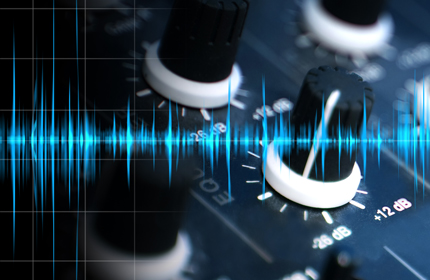
\includegraphics[width=\paperwidth,height=\paperheight]{pic1.jpg}};

  \end{tikzpicture}

   \vspace{0.5cm}
    \titlepage
  \end{frame}
}

\section
  {Постановка задачи}
\begin{frame}
  {Постановка задачи}

%   Things in a Bulleted List\pause

%   \begin{itemize}
%   \item Bullets that\pause
%   \item Come up\pause
%   \item One by one
%   \end{itemize}

  \begin{block}{Задача}
    Автоматическое распознавание жанра музыкального \\произведения 
  \end{block}
  Мотивация:
  \begin{itemize}
      \item У музыкальных жанров нет четких границ и характеристик
      \item Ручная разметка стоит дорого
      \item Широкий спектр применений: поиск, сортировка музыки
      \item Pandora, Spotify
  \end{itemize}
  
\end{frame}



\section
  {Main Body}
\begin{frame}
  {Обзор методов}

Основой признакового пространства служат MFCC коэффициенты.

\begin{itemize}
      \item k-means, k-
      \item Ручная разметка стоит дорого
      \item Широкий спектр применений: поиск, сортировка музыки
      \item Pandora, Spotify
  \end{itemize}
  
  
\end{frame}

\begin{frame}
  {Equations}

  Equations are easy
  \begin{itemize}
  \item Just copy/paste equations\pause
  \item From the paper!
    \begin{equation*}
      \textbf{p}^* = \underset{\textbf{p}}{\arg\!\min}~\sum_{\textbf{x}}\left[ I(\textbf{W}(\textbf{x};\textbf{p})) - T(\textbf{x}) \right]^2
    \end{equation*}
  \end{itemize}
\end{frame}


\begin{frame}
  {Pictures}

  \begin{figure}[t]
    \centering
    % \includegraphics[height=\dimexpr11\textheight/16\relax]{ducks}
    \caption{Kissing ducks}
  \end{figure}
\end{frame}


\begin{frame}
  {A Movie}

  \begin{block}{Some block}
    \begin{itemize}
    \item Movies only seem to work in Adobe Reader
    \item Movie file is not embedded, it must be on the computer
    \end{itemize}
  \end{block}

  \begin{exampleblock}{Some more block}
    Movies only seem to work in Adobe Reader\par
    Movie file is not embedded, it must be on the computer
  \end{exampleblock}

  \begin{alertblock}{}
    Some text in here.
    \begin{itemize}
    \item Movies only seem to work in Adobe Reader
    \item Movie file is not embedded, it must be on the computer
    \end{itemize}
  \end{alertblock}
\end{frame}



\section
  {Conclusion}

\begin{frame}
  {Credits}

  \begin{itemize}
  \item Brought to you by Cédric Mauclair
  \item Please let me know about improvements!
  \item inspiration: \url{http://www.shawnlankton.com}... (in code)
  \end{itemize}
\end{frame}


\begin{frame}
  {Questions}

  \nocite{lorem,ipsum}
  \bibliographystyle{plain}
  \bibliography{demo}

\end{frame}

\end{document}

